\part{Statistiken}

Hier ein Überblick über die Menge an Code: 
\begin{center}
	\begin{tabular}{ | l | l | l | l | l |}
		\hline
		& Dateien & Leerzeilen & Kommentare & Code \\ \hline
		\textbf{main} & 108 & 2253 & 3841 & 9467 \\ \hline
		\textbf{test} & ?   & ? & ?  & ? \\ \hline
		\textbf{total} & ? & ? & ? & ? \\ \hline
	\end{tabular}
\end{center}

Hier ein Überblick über die Testabdeckung:

\begin{figure}[H]
	\centering
	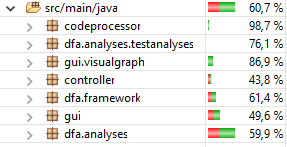
\includegraphics[width=0.8\textwidth]{Statistiken/coverage.png}
	\label{fig1}
\end{figure}


Hier wird lediglich die Abdeckung durch automatische Tests dargestellt. Zusätzlich dazu wurden noch manuelle Tests ausgeführt. Für die se stehen aber keine Überdeckungs-Statistiken zur Verfügung.